\tightsection{GO Overview and Challenges}

\comment{
\begin{packeditemize}
	\item System overview.
	\item Workflow of GO backend -- grouping, simplest form
	\item Limitations
\end{packeditemize}
}

\myparasum{Motivated by last section, we have built a real system} The trace-driven preliminary analysis in last section has shown that sharing client-side measurement to predict quality of a new session is feasible. Motivated by these results, we have implemented a working prototype called Video Global Optimization (GO) to realize the goal of accurately predicting the outcome of each decision by sharing measured quality samples from other clients in a {\it centralized} backend, and making best decisions for each session based on the prediction in order to actually improve video quality in the wild.

\myparasum{Organization of this section} This section begins with a design overview of GO. We also introduce the basic workflow of quality prediction and decision making in GO, and highlight the challenges faced by quality prediction algorithms. 


\tightsubsection{GO overview}

\begin{figure}[h!]
\centering
 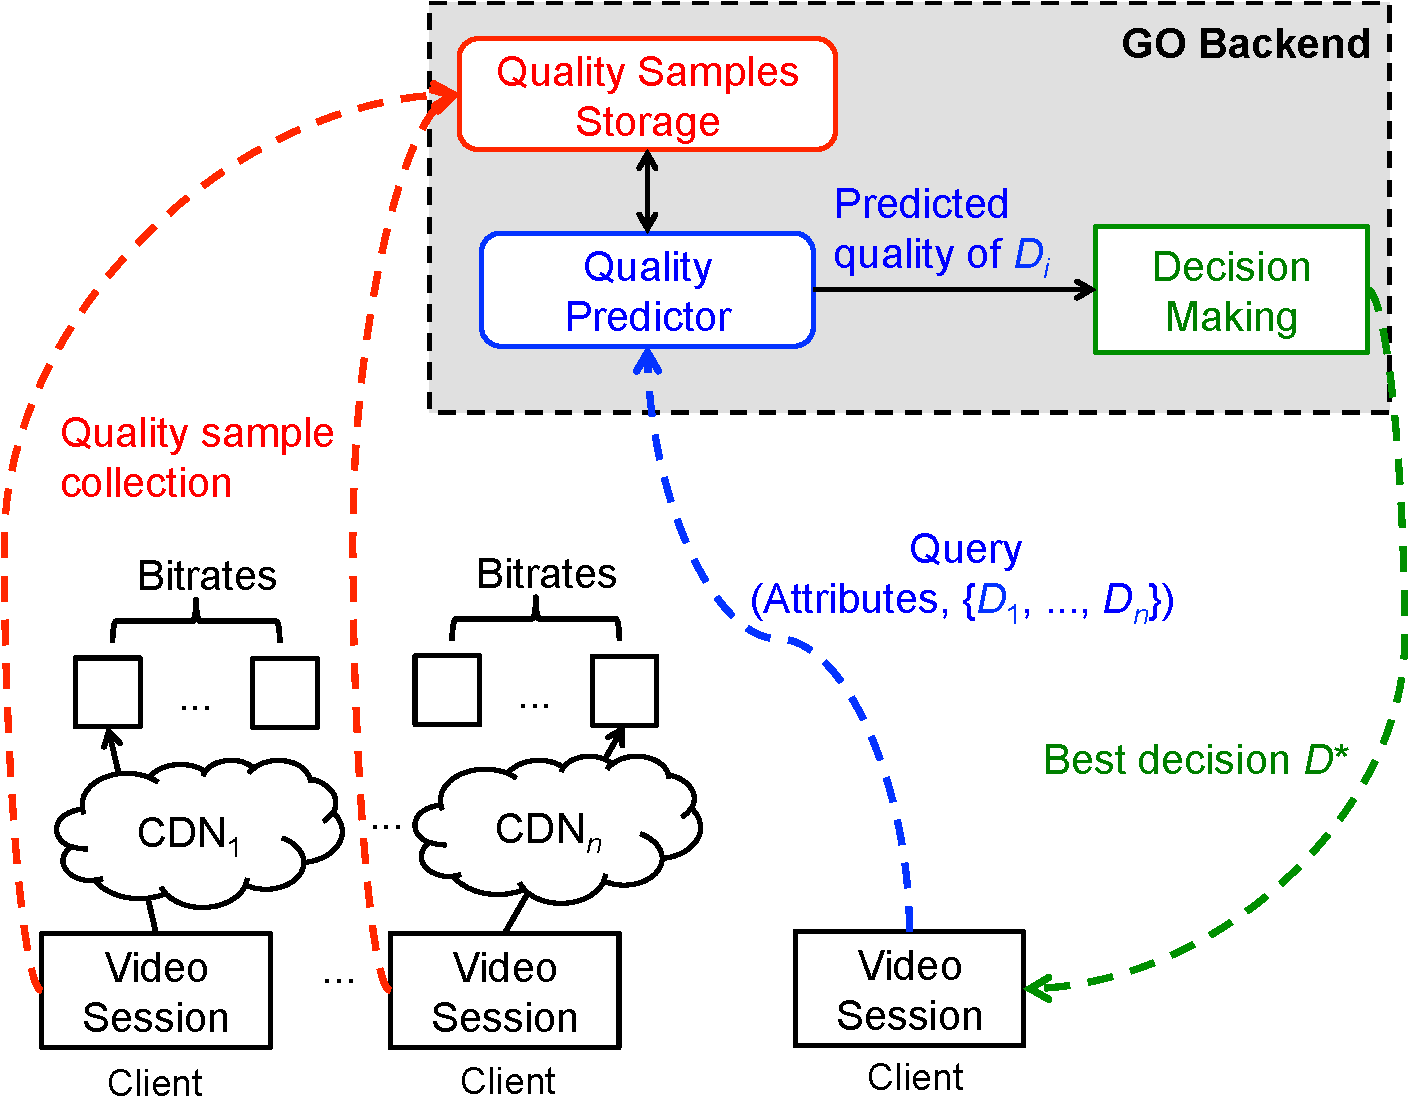
\includegraphics[width=0.5\textwidth] {figures/go-overview.pdf}
\tightcaption{Architecture of GO.}
\label{fig:go-overview}
\end{figure}

\myparasum{Highlevel components} Physically, in order to collect statistics from client and make decision in a centralized manner, GO has two parts: intrumentation code running within players during the cause of a video session at client-side, and GO backend running in publicly available clusters for centralized processing. Logically, there are three components of GO system (see Figure~\ref{fig:go-overview}). 

\myparatight{Quality sample collection} To collect feedback from client-side video sessions, the instrumentation code monitors the state of player and network condition, summarizes them in the form of quality samples (see details in \Section~\ref{subsec:dataset}) and send the quality samples back to GO backend for storage. Quality samples are then stored in a Hadoop File System for storage. \jc{in reality, the raw input from client is in log format of heartbeat, and later processed into quality samples by the backend. we may decide whether to expose it in scalability section.}

\begin{figure}[h!]
\centering
 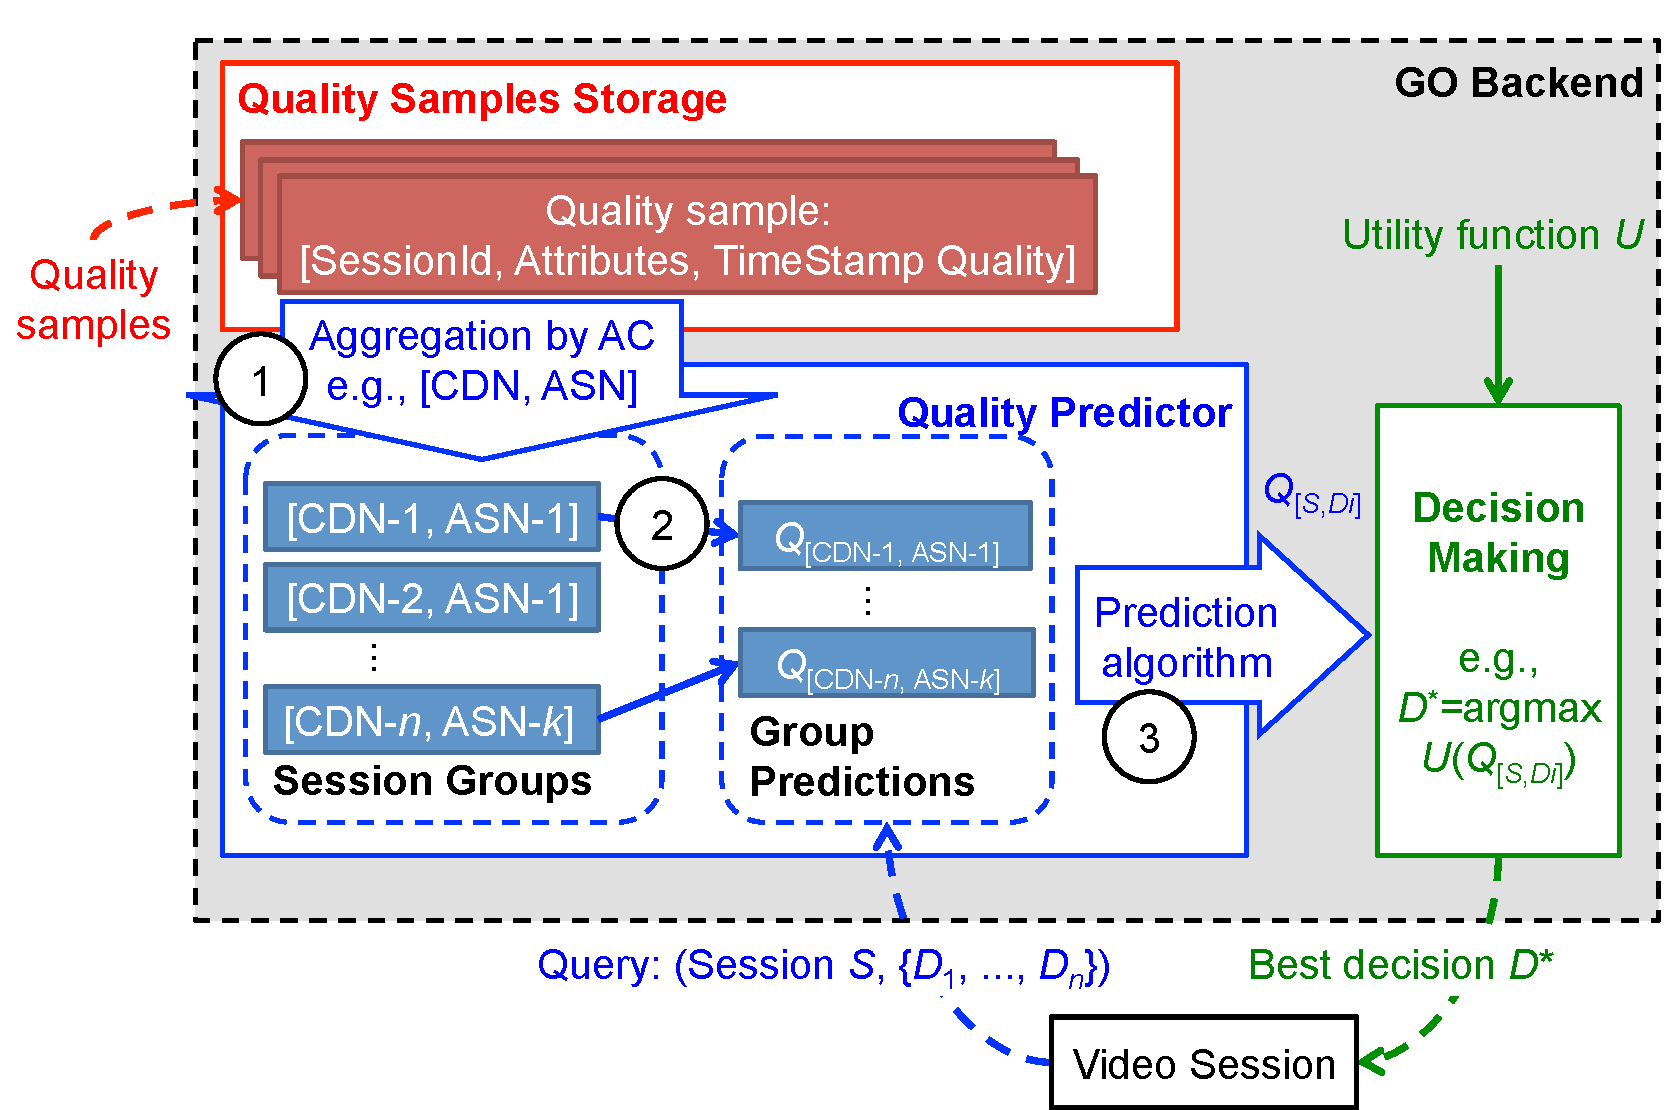
\includegraphics[width=0.5\textwidth] {figures/backend.pdf}
\tightcaption{Schematic overview of GO backend.}
\label{fig:backend}
\end{figure}

\myparatight{Quality prediction} Given a query for prediction on the quality of a session and one of its possible decision, the quality prediction uses the following three steps (see Figure~\ref{fig:backend}) to predict the outcome (quality) of the decision if it were to be used by the session at this moment.
\begin{packedenumerate}
	\item We aggregate together quality samples that share one or more attributes into {\it session group}s. The list of attributes used to aggregate samples is called {\it attribuet combination} (AC). Therefore, each session group is identified by an AC with value on each attribute. For example, if a session group is generated by aggregating by AC ``[CDN, ASN]'', the session group ``[$CDN-1, ASN-1$]'' describes all quality samples where the user belongs to $ASN-1$ and the session was assigned to a server from $CDN-1$.
	\item Each session group will generate a {\it group prediction} with respect to each quality metric. A simple way is to look at the mean of the quality of all samples within the group. The use of mean as prediction is motivated by  \Section~\ref{subsec:similarity} which shows that most quality values in a session group will not deviate too much away from the mean value of the group.
	\item A {\it prediction algorithm} is used to weight the group predictions, and merge them into the quality prediction of the query. The weight assigned to each group should reflect how similar this group is with the session in the query. For instance, given a query of a session that belongs to $ASN-1$, the group prediction of the session group $ASN-1$ should be given more weight than groups of other ASNs because its quality samples are supposed to be more similar to the queried session.
\end{packedenumerate}

\myparatight{Decision making} The best decision for a query will be determined based on the predicted quality of each metric and a utility function. A utility function can be a linear combination of multiple metrics or just one single metric. The choice of utility function is not the focus of this work. The best decision is then the one that gives the best utility function value given its predicted quality.



\tightsection{Video Quality Prediction Algorithms}
